\fancyhead[C]{Samuel Grace}

\section{Technology Strategy}

In this section, various techniques were applied to analyse the societal, business, user and customer needs relating to the multi-agent aerial landmine detection system. A SWOT matrix was used in Section \ref{sec:swot} to identify areas of strengths and possible opportunities, as well as potential weaknesses and threats that may arise. The aim of the SWOT matrix process was to convert weaknesses into strengths and threats into opportunities, which helps to meet the ultimate aims of any business: to survive and flourish in an ever-changing environment. In Section \ref{hoq}, a House of Quality was completed to enable the relationships between all of the significant needs to be analysed, understood and converted into actionable targets. The need for sustainable design is societal, with the needs below the roof being mostly technical/business-related and the remaining items constituting a mixture of customer and user needs. 


\subsection{SWOT Matrix}
\label{sec:swot}

An investigation into the \textbf{Strengths, Weaknesses, Opportunities and Threats (SWOT Analysis)} of the project's commercial viability was conducted in this section. The main goal of the exercise is to identify ways in which the weaknesses and threats can be converted into strengths and opportunities, respectively. The SWOT analysis is shown in Figure \ref{fig:swot}, using a template from Beretta.\footnote{Beretta: \url{mostlycolor.ch/2015/07/swot-matrices-in-latex.html}}

\begin{figure}[H]
\centering
\begin{tcbraster}[raster columns=2, boxrule=0mm, arc=0mm]
\begin{tcolorbox}[equal height group=A, size=fbox, colback=swotS!60, colframe=swotS!80!black, title=\textsc{\textbf{STRENGTHS}}]
\begin{itemize}
    \item Cutting-edge technology
    \item High precision engineering design
    \item Unique solution
    \item Redundancy safety net
    \item Cost-effective landmine detection
\end{itemize}
\end{tcolorbox}
\begin{tcolorbox}[equal height group=A, size=fbox, colback=swotW!60, colframe=swotW!80!black, title=\textsc{\textbf{WEAKNESSES}}]
\begin{itemize}
    \item Susceptibility to adverse weather conditions
    \item Limited production capacity
    \item Patents not yet obtained
    \item Reliance on sensor manufacturers
    \item Requirement for GPS
\end{itemize}
\end{tcolorbox}
\begin{tcolorbox}[equal height group=A, size=fbox, colback=swotO!60, colframe=swotO!80!black, title=\textsc{\textbf{OPPORTUNITIES}}]
\begin{itemize}
    \item Future cost reductions
    \item Ongoing improvement in sensor technology
    \item Expanding market potential
    \item Patents and software licensing
    \item Economies of scale
\end{itemize}
\end{tcolorbox}
\begin{tcolorbox}[equal height group=A, size=fbox, colback=swotT!60, colframe=swotT!80!black, title=\textsc{\textbf{THREATS}}]
\begin{itemize}
    \item Intellectual property theft
    \item Emerging competition
    \item Trade sanctions
    \item Drone regulations and privacy concerns
    \item Vulnerability to hacking and signal jamming
\end{itemize}
\end{tcolorbox}
\end{tcbraster}
\caption{SWOT analysis of the multi-agent aerial landmine detection business, template from Beretta.}
\label{fig:swot}
\end{figure}


\subsection{House of Quality}
\label{hoq}

The House of Quality forms part of a larger design philosophy, namely the Quality Function Deployment process, which ensures that all of the relevant needs are thoroughly considered during the engineering design process. The House of Quality shown in Figure \ref{fig:hoq} outlines the relationships between the societal, user, business and customer needs. The process involves analysing the interrelationships of the business needs in the roof of the house shown in Figure \ref{fig:hoq} and then considering how these needs correlate with the remaining needs. The exact method followed is described in \cite{chanqfd}. The competing product used as a reference was the MK Destiny\footnote{MK Destiny: \url{minekafon.org/index.php/destiny}}, and the House of Quality was adapted from an existing {\LaTeX} template.\footnote{{\LaTeX} template: \url{tex.stackexchange.com/questions/477795}}




\begin{figure}[H]
\centering
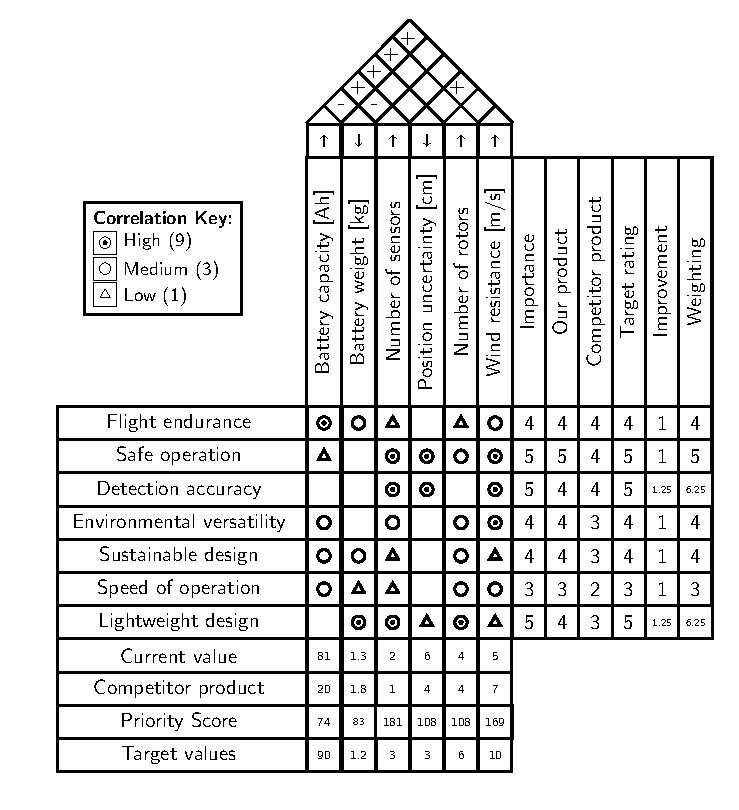
\includegraphics[width=0.79\textwidth]{figs/Samuel/Figures/test (2).pdf}
\caption{House of Quality}
\label{fig:hoq}
\end{figure}

% \subsection{Strengths}

% \begin{itemize}
%     \item \textbf{Cutting-edge technology:} the advanced state of the art technologies utilised in the design solution are likely to generate a significant amount of interest from potential customers. The product offered is unsurpassed in terms of optimal specifications for aerial landmine detection, which is a key competitive advantage.
    
%     \item \textbf{Highly skilled engineering design  team:} the product's greatest strength is the team of engineers working both individually and collaboratively to ensure that the design solution is exceptional. The strength of the team will both contribute to sales performance, as well as attracting funding from venture capitalists, since they are investors in people not ideas.
    
%     \item \textbf{Unique design solution:} to the best of the author's knowledge, the combination of techniques discussed in this report provides a unique design solution, with no other products leveraging the combination of technologies used here.
    
%     \item \textbf{Built-in redundancy:} the drone has failsafe measures built into the product to avoid unintended and undesirable outcomes. For example, the drone is designed to minimise the risk of it crashing in an unrecoverable position over a minefield. This feature will boost customer confidence.
    
%     \item \textbf{Cost-effective landmine detection:} the proposed design solution offers significant economic benefits compared to conventional methods for detecting landmines,  with less sophisticated UAV-based technology already cheaper than current detection options\cite{wef_landmine_drone_2016}.
% \end{itemize}

% \subsection{Weaknesses}
% \begin{itemize}
%     \item \textbf{Susceptibility to adverse weather conditions:} one of the product's key limitations is its ability to cope with adverse weather. Despite the drone having been made as resistant to wind conditions as possible, there still exists a threshold beyond which it is unsafe to operate a drone. Also, the landmine thermal detection ceases to work over frozen ground.
    
%     \item \textbf{Availability of skilled personnel:} there exists a severely limited supply of the highly specialised staff needed to produce the product. This is itself a limiting factor in the potential to produce and support high numbers of drones and the speed at which drone manufacture and testing can take place.
    
%     \item \textbf{Patents not yet obtained:} the software and hardware used for the design are not yet patented. Therefore, the product is not protected by UK Intellectual Property Law and is at risk of being sold by competitors.
    
%     \item \textbf{Reliance on sensor manufacturers:} the company's dependency on sophisticated sensor manufacturers has the potential to negatively impact productivity if there is a disruption or delay in the supply chain of these vital components
    
%     \item \textbf{Requirement for GPS:} the drone requires a GPS signal to operate effectively while on a mission. GPS signals can be blocked during times of conflict, however this issue is not a major concern since the product is focused on post-conflict demining operations.
% \end{itemize}

% \subsection{Opportunities}
% \begin{itemize}
%     \item \textbf{Future cost reductions:} the average cost of the components used in the drone have exhibited a decreasing trend of their price over time as technology develops. This decrease opens up the opportunity for increased profit margins and greater productivity because initial outlay on components will go further.
    
%     \item \textbf{Ongoing improvement in sensor technology:} this improvement will have a positive impact on the quality of drone produced. A key aspect of the business plan is to research and utilise new technology to optimise product performance, thereby enhancing its desirability.
    
%     \item \textbf{Expanding market potential:} the growing international awareness of the use of landmines and their consequences is prompting more governments and organisations to use available technology to locate and deactivate these devices. Landmine-detecting drones are a reliable, safe, cost-effective solution to the problem.
    
%     \item \textbf{Patents and software licensing:} it would be possible to patent the design of the drone, thus granting the company a sanctioned monopoly for a period of time. Also, since the software designed is used for a technical purpose (drone operation), it is possible to patent the software and license it to other companies for a fee, thus opening up another potential revenue source. 
    
%     \item \textbf{Economies of scale:} the product involves many bespoke components which become justified when the drone is manufactured at scale, since this approach then becomes cheaper than purchasing commercial off the shelf (COTS) components. 
% \end{itemize}

% \subsection{Threats}
% \begin{itemize}
%     \item \textbf{Intellectual property theft:} the drone's hardware and software designs could be stolen by competitors. Having the software closed-source mitigates this, and having a motivated engaged team minimises the risk of disclosure.
    
%     \item \textbf{Emerging competition:} there is likely to be competition from businesses developing landmine detecting drones using similar methods. An ongoing commitment to improvement and innovation is essential to remaining ahead in the market where new technologies are always likely to be emerging.
    
%     \item \textbf{Trade sanctions:} in any business that does not manufacture every component itself there is the risk of being let down by suppliers of individual components. Such disruptions in the supply chain would directly threaten production and likely lead to failure to meet deadlines and breaches of terms in a supply contract. This can be costly and lead to customers going elsewhere.
    
%     \item \textbf{Drone regulations and privacy concerns:} in the future, legal restrictions on the use of drones are likely to increase, firstly to ensure the safe use of drones and secondly to protect the privacy of citizens. Any tightening of drone regulations has the potential to adversely affect a business that supplies and manufactures drones. However, a business that can innovate and develop its product to guarantee that it is always complying with regulations is in a strong marketing position.
    
%     \item \textbf{Vulnerability to hacking and signal jamming:} the drones are vulnerable to being hacked or jammed by malicious actors. This threat is minimised by operating the drones in post-conflict scenarios.
    
% \end{itemize}




